% HW1 for Intro to Data Science
% also my first real foray into LaTeX ._.

\documentclass{article} 
\usepackage{fancyhdr, titling, graphicx}
\pagestyle{fancy}

% put name and page number in header
\fancyhead[L]{Green, Ben}
\fancyhead[R]{Page \thepage}

\author{Ben Green}
\title{Intro to Data Science HW 1}

\begin{document}

% title page
\begin{titlepage}
	\begin{center}
	\textsc{\LARGE Intro to Data Science HW 1}\\
	\vspace{3mm}
	
	{\large \theauthor}\\
	
	\tableofcontents
	\setcounter{secnumdepth}{0}
	\vfill
	
	{\large \today}
	\end{center}

\end{titlepage}

\section{Question 1}

\subsection{1a.}
\begin{table}[h]
\begin{center}
\begin{tabular}{ll}
Feature Name                                    & Feature Type                  \\ \hline
\multicolumn{1}{|l|}{\texttt{producer}}                  & \multicolumn{1}{l|}{nominal}  \\ \hline
\multicolumn{1}{|l|}{\texttt{release\_to\_review\_time}} & \multicolumn{1}{l|}{interval} \\ \hline
\multicolumn{1}{|l|}{\texttt{used\_real\_name}}          & \multicolumn{1}{l|}{binary}   \\ \hline
\multicolumn{1}{|l|}{\texttt{verified\_purchase}}        & \multicolumn{1}{l|}{binary}   \\ \hline
\multicolumn{1}{|l|}{\texttt{rating}}                    & \multicolumn{1}{l|}{{ordinal}}  \\ \hline
\multicolumn{1}{|l|}{\texttt{helpfulness}}               & \multicolumn{1}{l|}{ordinal}  \\ \hline
\multicolumn{1}{|l|}{\texttt{number\_of\_votes}}         & \multicolumn{1}{l|}{ratio}    \\ \hline
\multicolumn{1}{|l|}{\texttt{length\_of\_review\_text}}  & \multicolumn{1}{l|}{ratio}    \\ \hline
\end{tabular}
\end{center}
\end{table}

\subsection{1b.}
The mode of \texttt{producer} is Apple, with 4480 entries.

\subsection{1c.}
5077/9585, or 53\% of reviewers used their real name and had a verified purchase.

\subsection{1d.}
5077/13989, or 36\% of reviews with a verified purchase had a reviewer who used their real name.

\subsection{1e.}
\begin{table}[h]
\begin{center}
\begin{tabular}{|l|l|}
\hline
\textbf{Measure} & \textbf{Value} \\ \hline
min              & -537           \\ \hline
q1               & 74             \\ \hline
median           & 144            \\ \hline
max              & 11686          \\ \hline
interquartile    & 215            \\ \hline
\end{tabular}
\end{center}
\end{table}
These numbers can be displayed conveniently in a boxplot.

\subsection{1f.} 
\begin{center}
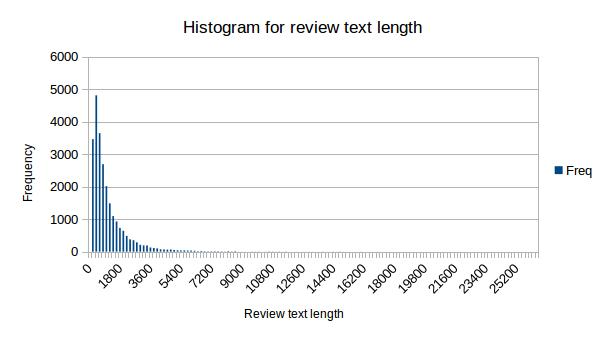
\includegraphics[keepaspectratio, scale=0.5]{histogram2.jpg}
\end{center}

\subsection{1g.}
Yes, the distribution of \texttt{length\_of\_review\_text}  is heavily skewed towards the shorter end. There are outliers of 26332, 1, and 1?

\subsection{1h.}
The Pearson correlation value between \texttt{length\_of\_review\_text} and \texttt{helpfulness} is approximately .25. This indicates that there is a slight positive correlation between these two variables.

\subsection{1i.}
\begin{center}
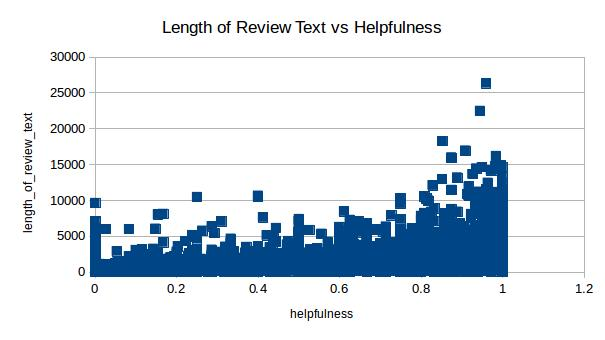
\includegraphics[keepaspectratio, scale=0.5]{scatter.jpg}

\section{Question 2}


\end{center}

\end{document}